%\documentclass[landscape,a0paper,fontscale=0.285]{baposter} % a0 is 841mm x 1189mm
\documentclass[landscape,archE,fontscale=0.285]{baposter} % archE is 36in x 48in

% Define colors from UT web page
\selectcolormodel{RGB}
%\definecolor{utburntorange}{cmyk}{0,0.2549,0.3922,0.03529}
\definecolor{burntorange}{RGB}{191,87,0}
\definecolor{rightfooterorange}{RGB}{248,151,31}
\definecolor{pms432}{RGB}{51,63,72}
\definecolor{pms7469}{RGB}{0,95,134}
\definecolor{pms7572}{RGB}{214,210,196}
\definecolor{pms7543}{RGB}{156,173,183}


\usepackage{graphicx} % Required for including images
\graphicspath{{./shared_figures/}{./figures/}}

\usepackage{graphbox}
\usepackage{overpic}

\usepackage{hyperref}
\hypersetup{
  colorlinks=true,
  urlcolor=pms432,
  pdftitle={Pecos Poster Template},
}

\usepackage{listings}
\lstset{numbers=left,
  basicstyle=\tiny\ttfamily,
  keywordstyle=\color{blue},
  breaklines=true,
  showtabs=false,
  showstringspaces=false,
  xleftmargin=2.5em,
}

\usepackage{amsmath} % For typesetting math
\usepackage{amssymb} % Adds new symbols to be used in math mode

\usepackage{booktabs} % Top and bottom rules for tables
\usepackage{enumitem} % Used to reduce itemize/enumerate spacing
\usepackage{palatino} % Use the Palatino font
\usepackage[font=small,labelfont=bf]{caption} % Required for specifying captions to tables and figures

\usepackage{multicol} % Required for multiple columns
\setlength{\columnsep}{1.5em} % Slightly increase the space between columns
\setlength{\columnseprule}{0mm} % No horizontal rule between columns

\usepackage{tikz} % Required for flow chart
\usetikzlibrary{shapes,arrows} % Tikz libraries required for the flow chart in the template

\newcommand{\compresslist}{ % Define a command to reduce spacing within itemize/enumerate environments, this is used right after \begin{itemize} or \begin{enumerate}
\setlength{\itemsep}{1pt}
\setlength{\parskip}{0pt}
\setlength{\parsep}{0pt}
}

\newcommand{\ud}{\,\mathrm{d}}
\newcommand{\vect}[1]{\boldsymbol{#1}}
\usepackage{mleftright}
\newcommand{\of}[1]{\mleft( #1 \mright)}\newcommand{\ddt}[1]{\partial_t #1}
\newcommand{\vth}{v_\textrm{th}}
\newcommand{\reals}{\mathbb{R}}
\newcommand{\RR}{\mathbb{R}}
\newcommand{\vr}{v}
%\newcommand{\vtheta}{\theta_{\vect{v}}}
%\newcommand{\vphi}{\varphi_{\vect{v}}}
%\newcommand{\vr}{v_{r}}
\newcommand{\vtheta}{v_{\theta}}
\newcommand{\vphi}{v_{\varphi}}
\newcommand{\vomega}{v_{\omega}}
\newcommand{\vrunit}{\hat{\vect{v}}_{r}}
\newcommand{\vthetaunit}{\hat{\vect{v}}_{\theta}}
\newcommand{\vphiunit}{\hat{\vect{v}}_{\varphi}}
\newcommand{\lp}[2]{L^{(#1)}_{#2}}
\newcommand{\lph}[2]{\tilde{L}^{(#1)}_{#2}}
\newcommand{\bfun}[2]{\Phi^{(#1)}_{#2}}
\newcommand{\tfun}[2]{\Psi^{(#1)}_{#2}}
\newcommand{\nfun}[2]{N^{(#1)}_{#2}}
\newcommand{\maxp}[2]{P^{(#1)}_{#2}}
\newcommand{\lagp}[2]{L^{(#1)}_{#2}}
\newcommand{\diffm}[3]{D^{(#1)}_{#2,#3}}
\newcommand{\planck}{h}
\newcommand{\te}{{\tilde{e}}}
\newcommand{\myint}{\int\limits}
\newcommand{\diff}[1]{\, d#1}
\usepackage{xcolor}
\usepackage{soul}
\newcommand{\mathcolorbox}[2]{\colorbox{#1}{$\displaystyle #2$}}

\usepackage{enumitem}
\setlist{itemsep=0pt}

\begin{document}

\begin{poster}
{
columns=4, % number of columns (change to suite your needs)
headerborder=closed, % Adds a border around the header of content boxes
colspacing=1em, % Column spacing
bgColorOne=white, % Background color for the gradient on the left side of the poster
bgColorTwo=white, % Background color for the gradient on the right side of the poster
borderColor=burntorange, % Border color
headershade=plain,
headerColorOne=burntorange, % Background color for the header in the content boxes (left side)
headerColorTwo=burntorange, %burntorange, % Background color for the header in the content boxes (right side)
headerFontColor=white, % Text color for the header text in the content boxes
boxColorOne=white, % Background color of the content boxes
textborder=roundedleft, % Format of the border around content boxes, can be: none, bars, coils, triangles, rectangle, rounded, roundedsmall, roundedright or faded
eyecatcher=false, %true, % Set to false for ignoring the left logo in the title and move the title left
headerheight=0.09\textheight, % Height of the header
headershape=roundedright, % Specify the rounded corner in the content box headers, can be: rectangle, small-rounded, roundedright, roundedleft or rounded
headerfont=\Large\bf\textsc, % Large, bold and sans serif font in the headers of content boxes
%textfont={\setlength{\parindent}{1.5em}}, % Uncomment for paragraph indentation
linewidth=2pt % Width of the border lines around content boxes
}
%----------------------------------------------------------------------------------------
% TITLE SECTION (spans whole width)
%----------------------------------------------------------------------------------------
%
{}
{\bf\textsc{Deterministic PG Boltzmann Solver I: \\{Collisional Term Discretization} }\vspace{0.5em}} % Poster title
{\textsc{Milinda Fernando, Daniil Bochkov  \hspace{12pt} The University of Texas at Austin}} % Author names and institution
{%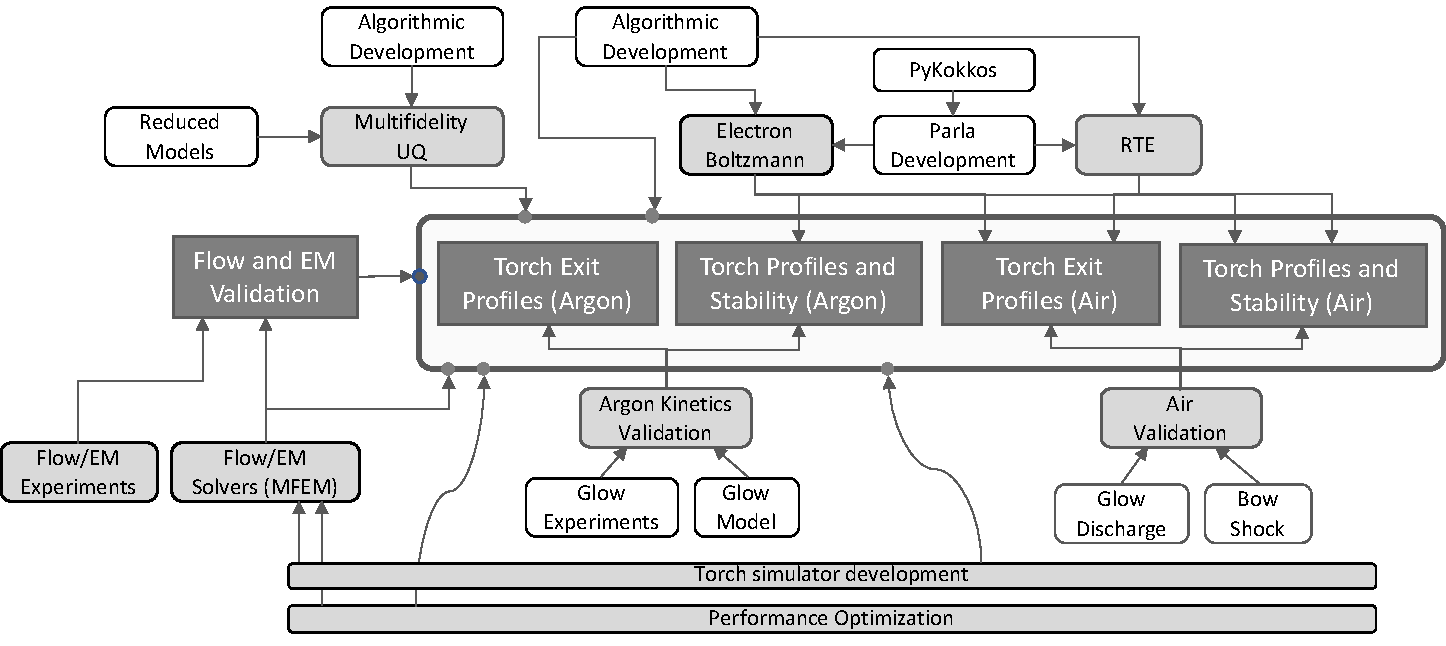
\includegraphics[align=c,height=0.09\textheight]{pecos_roadmap_tst_1.5.pdf}% just figure (must edit fig to add highlight box)
\raisebox{-0.5\height}{\begin{overpic}[height=0.09\textheight]{{pecos_roadmap_tst_1.5}.pdf} % figure + highlight box
    \put(38,32){\filldraw [semithick, fill=rightfooterorange, fill opacity=0.1, draw=gray, rounded corners] (0,0) rectangle (1.1,0.65);}
\end{overpic}}%
\hspace{12pt} \includegraphics[align=c,height=3em]{psaap3-logo.png}%
\hspace{12pt} \includegraphics[align=c,height=3em]{oden_pecos_2020_wordmark.png}%
}

%----------------------------------------------------------------------------------------
%	OBJECTIVES
%----------------------------------------------------------------------------------------

\headerbox{Objectives}{name=objectives,column=0,row=0}{

\begin{itemize}[leftmargin=*]
\item[--] Electron density function $f = f(\vect{x}, \vect{v}, t)$ defines transport and kinetic properties of plasma
\item[--] Need to couple plasma model with electron kinetics (planned for Y3)
\item[--] \textbf{Y2 Goal:} Extend standalone electron Boltzmann solver from Y1 to support spatially inhomogeneous case and additional inelastic collisions
\item[--] \textbf{Poster focus:} discretization of collisional term
\end{itemize}

\vspace{6.5em} % When there are two boxes, some whitespace may need to be added if the one on the right has more content
}

%----------------------------------------------------------------------------------------
%	INTRODUCTION
%----------------------------------------------------------------------------------------

\headerbox{Introduction}{name=introduction,column=1,row=0,bottomaligned=objectives}{

\begin{itemize}[leftmargin=*]
\item[--] \textbf{Boltzmann equation}
\begin{align*}
\partial_t f + \vect{v}\cdot \nabla_{\vect{x}} f  - \vect{E} \cdot \nabla_{\vect{v}}f = \overbrace{\mathcolorbox{green}{\sum_{a} C_a(f)}}^{\text{focus}}
\end{align*}
for example, $a=$ elastic collisions:
\begin{align*}
C_a(f) &= n_0\int_{S^2} v \underbrace{\sigma_a(v,\omega)}_{\tiny\text{\tiny scat. cross sec.}} 
\left( f(v^\prime) - f(v) \right) d \omega 
\end{align*}
\item[--] \textbf{Main challenge}: 6+1 dimensions
\item[--] \textbf{Overall approach}: FEM in $\vect{x}$, spectral in $\vect{v}$
\item[--] \textbf{Collisional Term}: Choice of basis?

%\item[--] \textbf{Spatially homogeneous case with acceleration term}
%\begin{align*}
%\partial_t f  - \vect{E} \cdot \nabla_{\vect{v}}f = \sum_{a} C_a(f)
%\end{align*}
\end{itemize}


}

%----------------------------------------------------------------------------------------
%	RESULTS 1
%----------------------------------------------------------------------------------------

\headerbox{Results}{name=results,column=2,span=2,row=0}{

\begin{multicols}{2}
\begin{itemize}[leftmargin=*]
\item[--] Cross section graph\\
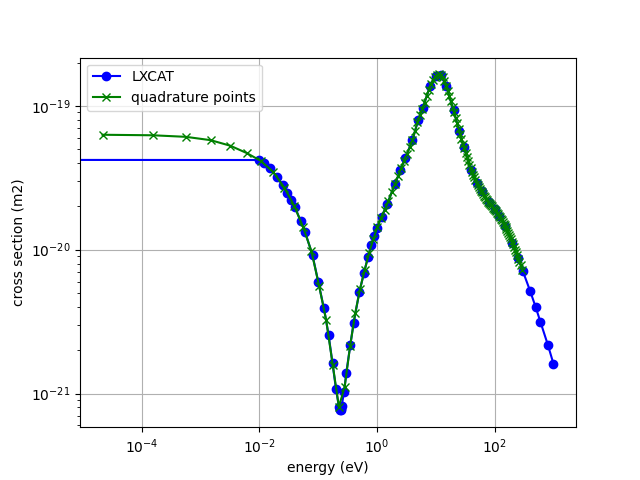
\includegraphics[width=.45\textwidth]{img/g0_tcs}
\item[--] Convergence of Maxwell polynomials\\
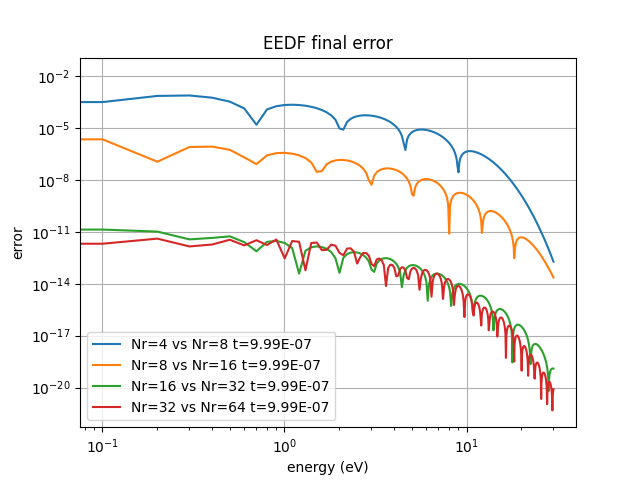
\includegraphics[width=.45\textwidth]{img/g0_mw_m0_eedf_final_error}
\end{itemize}
\columnbreak
\begin{itemize}[leftmargin=*]
\item[--] Mass conservation (?)\\
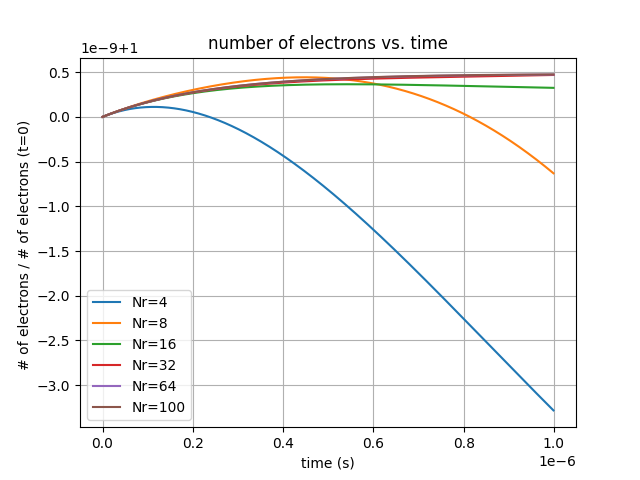
\includegraphics[width=.45\textwidth]{img/g02_mw_mass}
\item[--] Convergence of B-splines\\
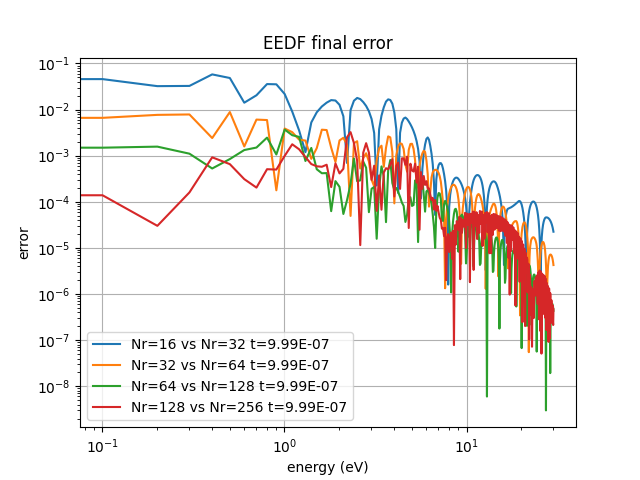
\includegraphics[width=.45\textwidth]{img/g0_bs_eedf_final_error}
\end{itemize}
\end{multicols}


}

%----------------------------------------------------------------------------------------
%	REFERENCES
%----------------------------------------------------------------------------------------

%\headerbox{References}{name=references,column=0,above=bottom}{
%
%\renewcommand{\section}[2]{\vskip 0.05em} % Get rid of the default "References" section title
%\nocite{*} % Insert publications even if they are not cited in the poster
%\small{ % Reduce the font size in this block
%\bibliographystyle{unsrt}
%\bibliography{sample} % Use sample.bib as the bibliography file
%}}

%----------------------------------------------------------------------------------------
%	CONTACT INFORMATION
%----------------------------------------------------------------------------------------

%%% \headerbox{Contact Information}{name=contact,column=3,aligned=references,above=bottom}{ % This block is as tall as the references block
%%% \begin{description}\compresslist
%%% \item[Web] www.university.edu/smithlab
%%% \item[Email] john@smith.com
%%% \end{description}
%%% }

%----------------------------------------------------------------------------------------
%	CONCLUSION
%----------------------------------------------------------------------------------------

\headerbox{Conclusion}{name=conclusion,column=2,span=2,row=0,below=results}{
\begin{itemize}[leftmargin=*]
\item[--] Analytical cross sections are needed to preserve convergence
\item[--] Maxwell polynomials are expected to converge faster (?)
\item[--] B-splines represent tails better (?)
\item[--] Tensorized assembly accelerates execution by several order of magnitudes
\end{itemize}
}

%----------------------------------------------------------------------------------------
%	FUTURE RESEARCH
%----------------------------------------------------------------------------------------

\headerbox{Future Research}{name=futureresearch,column=2,span=2,row=0,below=conclusion}{ % This block is as tall as the references block
\begin{itemize}[leftmargin=*]
\item[--] Add recombination reactions
\item[--] Couple with electric field forcing term
\item[--] Extend to spatially inhomogeneous case
\end{itemize}

}


%----------------------------------------------------------------------------------------
%	MATERIALS AND METHODS
%----------------------------------------------------------------------------------------

\headerbox{Approach: Petrov-Galerkin}{name=method,column=0,below=objectives}{ % This block's bottom aligns with the bottom of the conclusion block
\begin{itemize}[leftmargin=*]
\item[--] Expansion in terms of spherical harmonics:
\begin{align*}
f\of{\vect{v}} = \sum_{k,l,m} h_{k,l,m} \of{t} \Phi_{kl}\of{v} \underbrace{Y_{lm}\of{v_\theta, v_\phi}}_{\tiny\text{sph. harm.}}
\end{align*}
\item[--] Choice of radial representation:
\begin{align*}
\Phi_{kl}\of{v} =
\begin{cases}
v^l B_{k}\of{v} & \text{(B-splines)} \\
v^l M\of{v} P_{kl}\of{v} & \text{(Maxwell poly.)}
\end{cases}
\end{align*}
\begin{align*}
M\of{v} = n_e \left( \frac{m}{2 \pi kT }\right)^{\frac32} e^{-\frac{mv^2}{2kT}}
\end{align*}
\item[--] Weak formulation:\\
\scalebox{0.99}{\vbox{
\begin{multline*}
\myint_{R^3} C \phi\of{\vect{v}_e} d{\vect{v}_e} 
=
n_0 \myint_{R^3} \myint_{S^2}
\sigma_a(v,\omega) v 
f_e\of{\vect{v}_e} 
\\ \times
\left(
\phi\of{\vect{v}_e^\text{post}\of{\vect{v}_e,\vect{\omega}}} 
- \phi\of{\vect{v}_e} 
\right) d{\vect{\omega}}
d{\vect{v}_e}
\end{multline*}}}

\item[--] Resulting system of ODEs:
\begin{align*}
\sum_{k,l,m} M_{p,q,s}^{k,l,m} \partial_t h_{k,l,m}\of{t} = \sum_{k,l,m}  L_{p,q,s}^{k,l,m} h_{k,l,m}\of{t}
\end{align*}
\scalebox{0.75}{\vbox{
where
\begin{multline*}
{L}_{k,l,m}^{p,q,s} = n_0 \int_{v_r} \int_{S^2} \int_{S^2}  
v^2 M(v_r) P_k \of{\frac{v_r}{\vth}} Y^{lm}\of{v_\theta, v_\phi} v_r\sigma(|v_r|,\chi) \\ \times   \left(
P_p\of{\frac{v^{\prime}_r}{\vth}} Y_{qs}\of{v^{\prime}_\theta, v^{\prime}_\phi} - 
P_p\of{\frac{v_r}{\vth}} Y_{qs}\of{v_\theta, v_\phi}
\right) d\omega d\omega_v dv 
\end{multline*}
}}
\end{itemize}

}

%----------------------------------------------------------------------------------------
%	RESULTS 2
%----------------------------------------------------------------------------------------

\headerbox{Tensorized Implementation}{name=results2,column=1,below=objectives,bottomaligned=method}{ % This block's bottom aligns with the bottom of the conclusion block
\begin{itemize}[leftmargin=*]
\item[--] Tensorized formulation
%\begin{align*}
%{L}_{k,l,m}^{p,q,s} &=P^{r\theta\phi}_{k} Y_{lm}^{r\theta\phi} \left( M^{r\theta\phi\chi\gamma} \left(P^{r\theta\phi\chi\gamma}_{p} (v^\prime_r)	Y^{r\theta\phi\chi\gamma}_{qs} (v^\prime_\theta,v^{\prime}_\phi) - P^{r\theta\phi\chi\gamma}_{p} (v_r)	Y^{r\theta\phi\chi\gamma}_{qs} (v_\theta,v_\phi) \right) W_\chi W_\gamma \right) W_\phi W_\theta W_r
%\end{align*}
\begin{align*}
{L}_{k,l,m}^{p,q,s} = P^{r\theta\phi}_{k} Y_{lm}^{r\theta\phi} \times &\ldots \times W_\phi W_\theta W_r
\\
&\uparrow
\\
M^{r\theta\phi\chi\gamma} \times&\ldots\times W_\chi W_\gamma
\\
&\uparrow
\\
P^{r\theta\phi\chi\gamma}_{p} (v^\prime_r)	Y^{r\theta\phi\chi\gamma}_{qs} (v^\prime_\theta,v^{\prime}_\phi) &- P^{r\theta\phi\chi\gamma}_{p} (v_r)	Y^{r\theta\phi\chi\gamma}_{qs} (v_\theta,v_\phi)
\end{align*}

\item[--] Tensors:
\begin{itemize}[leftmargin=*]
\small
\item[$\circ$] $S^{r\theta\phi\chi\gamma}_{r^\prime\theta^\prime \phi^\prime}$: Scattering velocity tensor, for each $v=(r,\theta,\phi)$ and scattering solid angle $(\chi,\gamma)$ computes $(r^\prime,\theta^\prime,\phi^\prime)$ scattered or newly created particle velocity
\item[$\circ$] $P^{r\theta\phi\chi\gamma}_{p}$: radial polynomial evaluated at differed velocity for given incident particle ($r,\theta,\phi,\chi,\gamma$)
\item[$\circ$] $Y^{r\theta\phi\chi\gamma}_{qs}$: $qs$ spherical harmonic mode evaluated differed particle direction for a given incident particle ($r,\theta,\phi,\chi,\gamma$)
\item[$\circ$] $M^{r\theta\phi\chi\gamma}$: Maxwellian times $v_r$ evaluated for the differed particle for a given incident particle ($r,\theta,\phi,\chi,\gamma$)
\item[$\circ$] $\sigma^{r\theta\phi\chi\gamma}$: differential cross section broadcasted on scattering cross section angles. 
\item[$\circ$] $P^{r\theta\phi}_{k}$: radial polynomials evaluated at radial quadrature points. 
\item[$\circ$] $Y_{lm}^{r\theta\phi}$: spherical harmonics evaluated angular quadrature points. 
\end{itemize}

\end{itemize}
}

%----------------------------------------------------------------------------------------

\end{poster}

\end{document}
